\section{Calendar Queue}
Ein Optimierungsansatz f�r das \ac{PES}-Problem ist die \ac{CQ}, 1988 vorgeschlagen von Randy Brown. In Anlehnung an einen Kalender, in den Termine eingetragen werden, gibt es in einer \ac{CQ} Tage (Buckets), die mehrere Events enthalten k�nnen, sowie Jahre, die aus einer Anzahl von Tagen bestehen. Die Buckets sind jeweils Zeiger auf eine (beliebig implementierte) Liste, in der die Events liegen. Zum \textit{enqueuen} muss der Bucket, in den das Event geh�rt durch die Formel
\begin{equation}
	bucket\_idx=\floor{\frac{t(e)}{bw}} mod M
\end{equation}
ermittelt werden, wobei $bucket\_idx$ der Zielbucket, $t(e)$ die Zeit des Events, $bw$ die aktuelle \textit{\aclu{bw}} (L�nge des Tages) und $M$ die Anzahl der Buckets im Jahr ist. Anschlie�end wird das Element in den ermittelten Bucket eingef�gt. Um zu \textit{dequeuen}, muss das kleinste Element aus dem aktuellen Bucket entfernt werden, wobei leere Buckets �bersprungen werden.
Um auch Events \textit{enqueuen} zu k�nnen, die mehr als ein Jahr (Gesamtanzahl an Buckets) in der Zukunft liegen, wird das Datum im Event selbst gespeichert, sodass dieses bei einer \textit{dequeue}-Operation in den vorigen Jahren �bersprungen werden kann. \cite{brown_cq}
\begin{figure}[htb]
    \centering
    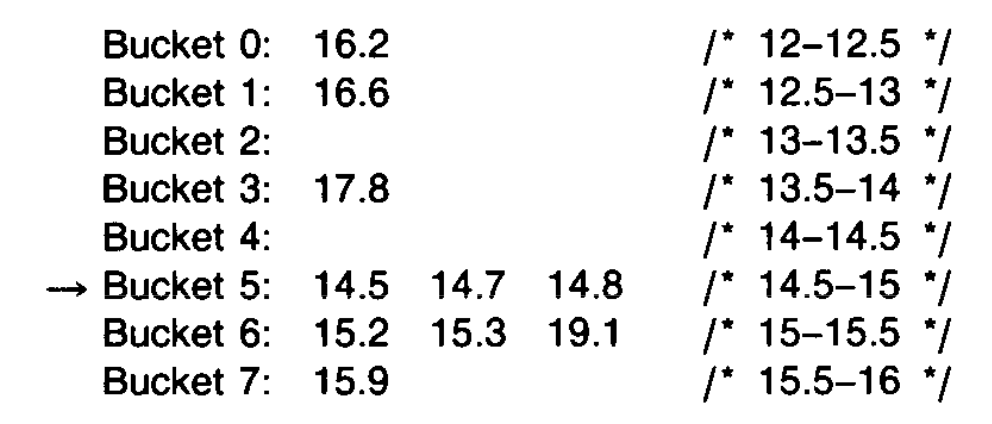
\includegraphics[width=0.4\textwidth]{images/cq}\caption{Calendar Queue - Struktur \cite{brown_cq}}\label{Calendar Queue - Struktur}
	Beispiel einer Calendar Queue mit Bucketbreite 0.5 und Jahresl�nge 8. Das Event zur Zeit 19.1 wird beim \textit{dequeuen} in diesem Jahr �bersprungen.
\end{figure}
\subsection{Optimierungen}
Die L�nge eines Jahres und die L�nge eines Tages werden dynamisch an die Anzahl der Events angepasst. Steigt die Zahl der Events auf mehr als das doppelte der Anzahl der Buckets, werden die Events in eine \ac{CQ} doppelter Gr��e kopiert, sodass durchschnittlich jedes Event in einem eigenen Bucket liegt. Analog halbiert sich die Gr��e der \ac{CQ} bei halb so viel Events wie Buckets in der \ac{CQ} vorhanden sind. Die \textit{\aclu{bw}} wird beim Vergr��ern/Verkleinern angepasst. Sie sollte ungef�hr so gro� sein, wie die durchschnittliche Zeit zwischen zwei benachbarten Events.
Eine von Brown vorgeschlagene Heuristik, eine akzeptable \textit{\acl{bw}} zu ermitteln, ist, die ersten \textit{n} Elemente zu \textit{dequeuen}, die durchschnittliche Zeit zwischen diesen Events zu errechnen, und diese anschlie�end wieder zu \textit{enqueuen}. In Bezug auf statistische Aussagekraft muss \textit{n} hinreichend gro� gew�hlt werden. \cite{brown_cq}
\subsection{Performance}
Die Calendar Queue hat eine theoretische Komplexit�t von $ O(1) $ f�r sowohl die \textit{dequeue}- als auch die \textit{enqueue}-Operation. 
Die amortisierte Zeit wird jedoch ma�geblich durch die Zeitverteilung der Events beeinflusst. W�hrend die Performance bei absoluter Gleichverteilung optimal ist, ist bei gro�er Varianz des Abstandes der Events zueinander keine konsistente Performance gegeben. Wenn sich Events innerhalb eines Buckets h�ufen, dauert das \textit{enqueuen} l�nger, da die \ac{LL} l�nger wird. Wenn viel Zeit zwischen den Events liegt, m�ssen viele leere Buckets untersucht werden, bevor das n�chste Element gefunden wird.  \cite{brown_cq}\cite{wuttisittikulkij_study_2003} \\
Brown schl�gt zur Behebung letzteren Problems eine Strategie vor, nach der nach einem eventfreien Jahreszyklus das kleinste Element von allen Buckets zur�ckgegeben wird. \cite{brown_cq}
\subsection{Erweiterung: Dynamic Calendar Queue}
In der \ac{DCQ} wird die Heuristik zur Berechnung von \textit{\ac{bw}} beim Kopieren in eine gr��ere bzw. kleinere Queue ver�ndert. Es werden nicht die ersten \textit{n} Elemente zur Berechnung der durchschnittlichen Zeit zwischen den Events genutzt, sondern Elemente aus dem Bucket, in dem die meisten Events sind. So soll ein repr�sentativeres Ergebnis der Zwischeneventzeit erzielt werden.
Au�erdem werden zwei Metriken eingef�hrt: Die durchschnittlichen \textit{enqueue}- und \textit{dequeue}-Kosten ($C_E$ und $C_D$). Wenn diese einen vorher definierten Grenzwert �berschreiten, wird eine Neuberechnung von \textit{\ac{bw}} initiiert, sodass sich die Queue an �nderungen in der Eventdistribution \textit{dynamisch} anpasst. \cite{dcq}\cite{snoopy}
